%---------------------------------------------------
%----- Calculation of the Root Hashes
%---------------------------------------------------
\subsection{Calculation of the Root Hashes}
Every root hash of a document $R_{\texttt{doc-root}}$ is stored in the
\textit{AnchorRepository} smart contract. The document root hash is calculated from three different Merkle trees (see Fig. \ref{fig:root-hash}). 
\subsubsection{Merkle Tree of Fields}
A Merkle tree is a way to calculate a unique hash from a set of items. We formally define a Merkle tree function $\mathcal{M}$ to calculate a root hash $R \in \mathbb{B}_{32}$ of document fields $F$. The implementation of the Merkle tree function is introduced in Sec. \ref{sec:precise_proofs}.
 \begin{eqnarray}
 R & = &\mathcal{M}(F_{[0]},...,F_{[n]}) \\
 R & \in & \mathbb{B}_{32}
\end{eqnarray}
\newline
\subsubsection{Schema Root and CoreDocument Root}
As a first step, we calculate the Merkle root of the schema fields $S$ and the core document fields $C$ of a document $d$\\\\
\textbf{Schema Root} The Merkle root of the document schema data, formally $R_{{\texttt{schema}}}$ 
\newline
\begin{equation}
    R_{{\texttt{schema}}} = \mathcal{M}(d_S)
\end{equation}
\newline
\textbf{CoreDocument Root} the Merkle root of the core document data, formally $R_{{\texttt{core}}}$ \\
\begin{equation}
R_\texttt{core} = \mathcal{M}(d_C)\\
\end{equation}
 \subsubsection{Signing Root}
The $R_{\texttt{signing}}$ is calculated from the SHA256 hash of the concatenated $R_\texttt{core}$ and $R_{\texttt{schema}}$
\newline
\begin{equation}
R_{\texttt{signing}} = \texttt{sha256}(R_\texttt{core}\| R_{\texttt{schema}})
\end{equation}\\
We formally define a helper function for calculating the $R_{\texttt{signing}}$ 
\begin{eqnarray}
R_{\texttt{signing}}& =&\mathsf{calculateSigningRoot}(d) \\
\mathsf{calculateSigningRoot}(d)& =& \texttt{sha256}(\mathcal{M}(d_C)\| \mathcal{M}(d_S))
\end{eqnarray}
 \subsubsection{Signatures Root}
 A Merkle root of the collaborator signature must be part of the document root hash $R_{\texttt{doc-root}}$. The signatures are relevant for the document consensus, explained in the following chapters. \\\\
\textbf{Signature Root} A signature root hash defines the Merkle root of all signatures $d_{\texttt{signatures}}$, formally $R_{\texttt{signatures}}$:
\newline
\begin{equation}
R_{\texttt{signatures}} = \mathcal{M}(d_{\texttt{signatures}})\\
\end{equation}
 \subsubsection{Document Root}
The final  document root hash $R_{\texttt{doc-root}}$ of the entire document $d$ is defined as the SHA256 hash of the concatenated signing root hash $R_{\texttt{signing}}$ and signature root hash $R_{\texttt{signatures}}$ 
\newline
 \begin{equation}
R_{\texttt{doc-root}} =  \texttt{sha256}(R_{\texttt{signing}}\|R_{\texttt{signatures}})
\end{equation}\\
A tree of the  $R_{\texttt{doc-root}}$ calculation. (see Fig. \ref{fig:root-hash})

%TODO (Manuel): Why sometimes R and D?

%All information related to the document is stored in a structured protobuf message called CoreDocument, \mathsf{CD}, along with a document-specific message, Data, \mathsf{D} such as an Invoice or PurchaseOrder. Both messages are serialized with precise proofs into \\mathsf{CD} 

\begin{figure}[thpb]
\centering
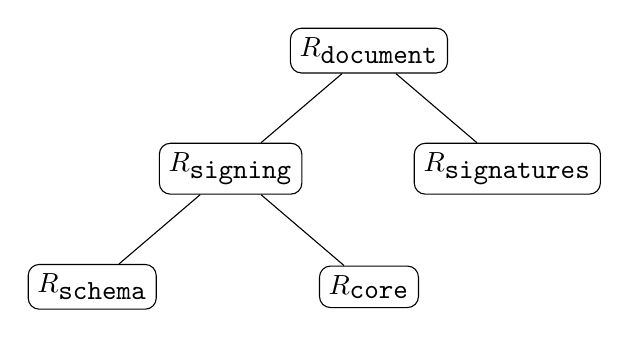
\begin{tikzpicture}[sibling distance=10em,
  every node/.style = {shape=rectangle, rounded corners,
    draw, align=center, %top color=white, bottom color=gray!20
    }]]
  \node {$R_{{\texttt{document}}}$}
    child { node {$R_{{\texttt{signing}}}$}  child { node {$R_{{\texttt{schema}}}$}
    } child { node {$R_{{\texttt{core}}}$}
    } }
    child { node {$R_{{\texttt{signatures}}}$}};
\end{tikzpicture}
\caption{Calculation of the document root hash} \label{fig:root-hash}
\end{figure}
We can define a second help function called $\mathsf{calculateDocumentRoot}(d)$ for calculating the entire $R_{\texttt{doc-root}}$. 
\begin{eqnarray}
R_{\texttt{doc-root}}& =&\mathsf{calculateDocumentRoot}(d) \\
\mathsf{calculateDocumentRoot}(d)& = & \texttt{sha256}( \mathsf{R_{\texttt{signing}}}\| \mathcal{M}_{\texttt{tree}}(d_S))
\end{eqnarray}
The functions $\mathsf{calculateDocumentRoot}(d)$ and $\mathsf{calculateSigingRoot}(d)$ are needed for the document consensus chapter.
%\begin{eqnarray}
%R_{\mathsf{CD}} = \mathcal{M}(\mathsf{CD}) \\
%R_{\mathsf{D}} = \mathcal{M}(\mathsf{D}) \\
%R_{\mathsf{S}} = \mathrm{sha256}(R_{\mathsf{CD}} + R_{\mathsf{D}}) \\
%$R = \mathcal{M}(R_{\mathsf{S}}, \mathbb{S}) \\
%\end{eqnarray}
% TODO: what is the correct operation for binary append?

% formula list
%sig_root = T(T(\textt{CoreDocument}), T(\textt{DocumentData}))
%Sig_alice = s(sig_root, private key alice)
%S = {s(sig_root, pk_alice), s(sig_root, pk_bob), ...} 
% document_root = T({sig_root, S})
